\documentclass[12pt,a4wide,oneside,
%twocolumn,landscape,
headings]{report}
\usepackage[utf8]{inputenc}
\usepackage[czech]{babel}
\usepackage[T1]{fontenc}
\usepackage{amsmath}
\usepackage{amsfonts}
\usepackage{amsthm}
\usepackage{hyperref}
\usepackage{multicol}
\usepackage{subcaption}
\usepackage{amssymb}
\setcounter{secnumdepth}{2}
\usepackage{amsmath}
\usepackage{upgreek}
\usepackage{makeidx}
\usepackage{graphicx}
\usepackage{tcolorbox}
\tcbuselibrary{theorems}
\usepackage{wrapfig}
\usepackage{amsmath}
\usepackage{pdfpages}
\definecolor{yourcolor}{RGB}{0, 120, 60}
\pagestyle{headings}
\usepackage{booktabs}
\newtheorem{veta}{Věta}[chapter]\theoremstyle{definition}
\newtheorem{defi}{Definice}[chapter]\theoremstyle{definition}
\newtheorem{prav}{Pravidlo}[chapter]\theoremstyle{definition}
\newenvironment{eq}{\begin{tcolorbox}[ams equation,colback=yourcolor!10!white,colframe=yourcolor]}{\end{tcolorbox}}


\usepackage[left=2cm,right=2cm,top=2cm,bottom=2cm]{geometry} 
\usepackage[pagestyles]{titlesec}
\titleformat{\chapter}[block]{\bfseries\Huge}{\thechapter}{10pt}{\vspace{-20pt}}[\vspace{-0.5ex}]

%\usepackage{blindtext}
\author{Jakub Dokulil}
\title{Matematika}
%\usepackage{a4wide}
%\usepackage[left=1.5cm,right=1.5cm,top=2cm,bottom=2cm]{geometry}
\begin{document}
\pagenumbering{Roman}
\maketitle
\begin{verse}
Tato příručka byla zpracována v souladu s tématy k školní části maturitní zkoušky na Gymnáziu Křenová.\\
Vysázeno pomocí systému \LaTeX.
\end{verse}
%\tableofcontents
\pagenumbering{arabic}

\chapter{Množiny}
Kartézský součin množin $A$ a $B$, je množina \textbf{všech} uspořádaných dvojic $\left[ x;y \right]$, ve kterých $x \in A$ a zároveň $y\in B$.

$$ A\times B=\lbrace\mathrm{všech} \left[x;y\right]; x\in A \wedge y\in B \rbrace $$
\begin{figure}[h!]
 \includegraphics[width=10cm]{souhrn/fce/bin_soucin.pdf}
 \centering
 \caption[kartézský součin graficky]{Jak ukazuje graf na obrázku, přímka zobrazující body se souřadnicí která nepatří množině je čárkovaná, každý bod na čárkované přímce nenáleží kartézskému součinu}
\label{fig:kartsoucin}
\end{figure}
\includepdf[pages=1,offset=0mm 0in]{zobrazeni}


\chapter{Výroková logika}
\textit{Výroková logika} je část matematiky zabývající se studiem výroků (jak jednoduchých tak složených) a posuzováním jejich pravdivosti, dokazatelnosti a vyvratitelnosti.
\section{Výroky}
Výrok je základní objekt zkoumání výrokové logiky.\\
\begin{quote}
\textit{\textsc{\textbf{Výrok}} je srozumitelná oznamovací věta, u níž lze jednoznačně rozhodnout zda-li je či není pravdivá.}
\end{quote}

Pravdivému výroku je přisuzována \textit{pravdivostní hodnota} 1.

Nepravdivému výroku je přisuzována \textit{pravdivostní hodnota} 0.
\begin{table}
	\begin{tabular}{lc|c}
	\multicolumn{2}{c|}{Výrok (popř jeho pravdivostní hodnota)} & Věty, jež nejsou výroky. \\ 
	\hline 
	3 je liché číslo & 1 & Otevřte si sešity! \\  
	$4 \mid 15$ & 0 & Je dnes čtvrtek? \\  
	Des je \today & 1 & \uv{Newtonův gravitační zákon} \\ 
	\end{tabular} 
	\caption{tabulka s příklady výroků}
	\label{tb:příklady výroků}
\end{table}\\
 \textsc{\textbf{Negace výroku $V$}} je výrok $V'$ nebo $\urcorner V$ který popírá jeho pravdivostní hodnotu. (Např slovy \uv{Není pravda že..})
\paragraph{Příklad}
$V$\ldots Matematika je věda.
$\urcorner V$\ldots Matematika není věda.
\subsection{Kvantifikované výroky}
\textsc{\textbf{Kvantifikovaný výrok}} je právě takový výrok, který obsahuje kvantifikátor. Kvantifikátor je slovo či slovní spojení udávající informaci o počtu.
\begin{enumerate}
\item \textbf{Existenční kvantifikátor}, jinak $\exists$ \ldots \textit{existuje alespoň jendno}\\
\textbf{Např.:} \emph{existuje alespoň jedno sudé číslo} \ldots $$\exists x \in \mathbb{N} ; 2\vert x$$
\item \textbf{Obecný kvantifikátor}, jinak $\forall$ \ldots \textit{pro všechna}\\
\textbf{Např.:} \emph{pro všechna reálná $x$} \ldots $$\forall x \in \mathbb{R}$$
\item \textbf{Upřesňující kvantifikátor} 
	\begin{itemize}
	\item \textit{Více (nebo rovno) než $n$ prvků}
	\item \textit{právě $n$ prvků}
	\item \textit{méně (nebo rovno) než $n$ prvků}
	\end{itemize}
\end{enumerate}
lze použít i jiné spojení jako např \textit{více \ldots ,méně \ldots,} atd.
\paragraph{negace výroků s kvantifikátory}
Řídí se pravidly:
\begin{table}[h!]
\begin{tabular}{p{5cm}c|p{5cm}c}
 
\multicolumn{2}{c|}{Výrok $V$} & \multicolumn{2}{c}{Negace výroku $\urcorner V$} \\  
\hline
Existuje $x$ z množiny $M$ s vlastností $V$ & $\exists x \in M; V(x)$ & Všechna $x$ z množiny $M$ nemají vlastnost $V$ & $\forall x \in M; \urcorner V(x)$\\  
Všechna $x$ z množiny $M$ mají vlastnost $V$ & $\forall x \in M; V(x)$ & Existuje $x$ z množiny $M$ které nemá vlastnost $V$ & $\exists x \in M; \urcorner V(x)$ \\  
\end{tabular}
\caption{Negace výroků s kvantifikátory}
\label{tb:negace_kvant_vyroku} 
\end{table}\\
Pravidla užitá na příkladech:\\
\begin{tabular}{ll|ll}
\multicolumn{2}{l|}{Výrok ($V$)} & \multicolumn{2}{l} {Negace výroku ($ \urcorner V$)} \\ 
\hline 
Existuje $x$ větší než 3. & $\exists x; x>3$ & Všechna $x$ jsou menší nebo rovny než tři. & $\forall x; x\leq 3$\\  
Všichni lidé jsou dokonalí. &  & Existuje dokonalý člověk. &  \\  
\multicolumn{2}{l|}{Máš nejvýš dvě možnosti.} & \multicolumn{2}{l}{Máš více jak dvě možnosti} \\  
\multicolumn{2}{l|}{Dal aspoň 3 góly.} & \multicolumn{2}{l}{Dal nejvýš dva góly. } \\ 
\multicolumn{2}{l|}{Máme alespoň 4, ale nejvýš 9 korun.} & \multicolumn{2}{l}{Mám méňe než čtyři nebo více jak 9 korun.} \\ 
\end{tabular} 

$$A \veebar B \Leftrightarrow \left(\neg A \wedge B\right)\vee \left(A \wedge \neg B\right)$$

\begin{table}

\begin{tabular}{p{3cm}l}
\toprule
výrok&negace výroku\\\midrule
$A$&$\neg A$\\
$A\vee B$&$\neg A \wedge \neg B$\\
$A \wedge B$&$\neg A \vee \neg B$\\
$A\veebar B$& $A\Leftrightarrow B$\\
$A\Rightarrow B$& $A \wedge \neg B$\\
$A\Leftrightarrow B$&$A \veebar B $\\
\bottomrule
\end{tabular}
\caption{Negace složených výroků}
\end{table}

\chapter{Algebraické výrazy a jejich úpravy}
\begin{defi} \textbf{Algebraický výraz} je zápis skládající se z čísel a z písmen označujících proměnné, jež jsou spojeny znaky operací, popř. obsahují
závorky.

\end{defi}

\begin{defi}\textbf{Definiční obor proměnných} je množina hodnot proměnných, pro něž má algebraický
výraz smysl

\end{defi}

Úprava algebraického výrazu spočívá v nahrazení daného algebraického výrazu
jednodušším algebraickým výrazem (ve tvaru např.
součinu, bez odmocnin ve jmenovateli, ...), který se mu
rovná ve společném definičním oboru proměnných

\begin{table}
\centering
\begin{tabular}{p{9.5cm}p{9.5cm}}
\toprule
$(a+b)^2=a^2+2ab+b^2$ & $a^2-b^2=(a+b)(a-b)$ \\ 

$(a+b)^3=a^3+3a^2b+3ab^2+b^3$ & $a^3-b^3=(a-b)(a^2+ab+b^2)$ \\ 
$(a+b+c)^2=a^2+b^2+c^2+2ab+2ac+2bc$ &$a^3 + b^3 =(a+b)(a^2-ab+b^2)$   \\další vzorce jdou odvodit pomocí bin. věty&$a^5+b^5=(a+b)(a^4-a^3b+a^2b^2-ab^3+b^4)$\\
\multicolumn{2}{p{\textwidth}}{
{\large $a^n+b^n=(a+b)(a^{n-1}-a^{n-2}b+a^{n-3}b^2-\cdots+b^{n-1})$ }
pro lichá $n$.}\\
\multicolumn{2}{p{\textwidth}}{{\large $a^n-b^n=(a-b)(a^{n-1}+a^{n-2}b+a^{n-3}b^2 +\cdots +b^{n-1})$} pro $n\in\mathbb{N}$} \\
\multicolumn{2}{p{\textwidth}}{{\large $ \left(a\pm b\right)^n = {n\choose 0} a^n\cdot b^0\pm {n\choose 1}a^{n-1}\cdot b^1+{n\choose 2} a^{n-2}\cdot b^2\pm\cdots+{n\choose n} a^{0}\cdot b^n $} pro sudá $n$}\\\multicolumn{2}{p{\textwidth}}{{\large $ \left(a\pm b\right)^n = {n\choose 0} a^n\cdot b^0\pm {n\choose 1}a^{n-1}\cdot b^1+{n\choose 2} a^{n-2}\cdot b^2\pm\cdots\pm{n\choose n} a^{0}\cdot b^n $} pro lichá $n$}\\
\bottomrule
\end{tabular}

\caption{Základní algebraické vzorce}
\end{table}

\chapter{Linearní rovnice a jejich soustavy}
\begin{defi} Lineární rovnicí s $n$ neznámými, $x_1 ,\, x_2 ,\,\dots, x_n$, nazýváme rovnici tvaru:
$$a_1 x_1 + a_2 x_2 + \ddots + a_n x_n = b, \;\mathrm{kde\:} a_i,\, b \in \mathbb{R},\,i\in\lbrace 1, 2, ... , n\rbrace.$$
\end{defi}


\chapter[Kvadratická rce]{Kvadratická rovnice a vztahy v ní}
\chapter{Kvadratické nerovnice}
\chapter{Iracionální rovnice a nerovnice}
\chapter{Rovnice a nerovnice s abs hodnotou}
\chapter{Další typy rovnic a nerovnic}
\chapter{Rovnice s parametrem}
Odvození vzorce pro výpočet kořenů kv. rce. Nechť je dána kvadratická rovnice $ax^2+bx+c=0$, $a\neq 0$, tedy lze jím vynásobit rovnici. 
$$a^2x^2+abx+ac=0 $$
Převede se $abx=2ax\frac{b}{2}$ a doplní se na druhou mocninu dvoučlenu výrazem $\left(\frac{b}{2}\right)^2$ ten je zapotřebí také odečíst.
$$\underbrace{(ax)^2 + 2ax\frac{b}{2}+\left(\frac{b}{2}\right)^2}_{\mathrm{vzorec}\,(a+b)^2} -\left(\frac{b}{2}\right)^2 +ac=0$$
$$\left(ax+\frac{b}{2} \right)^2-\frac{b^2}{4}+ac=0\;/\cdot4 $$
$$4\left(ax+\frac{b}{2} \right)^2-b^2+4ac=0 $$ 
První člen se roznásobí a vytkne se $(-1)$.
$$\left(2ax+b \right)^2 -\left(b^2-4ac \right)=0$$
$$\left(2ax+b \right)^2 =\left(b^2-4ac \right)$$
1) $b^2-4ac>0$, úpravami vzniká vzorec
\begin{eq}
x_{1,2}=\frac{-b\pm\sqrt{b^2-4ac}}{2a}
\end{eq}
2) $b^2-4ac=0$, pak 
\begin{eq}
x_{1,2}=\frac{-b}{2a}
\end{eq}

\chapter{Pravoúhlý trojúhelník}
\chapter{Shodná zobrazení}

Zobrazení je aková binární relace, která přiřazuje každému prvku z množiny $A$ (prvkem může být také například bod, přímka, úsečka) nejvýše jeden prvek z množiny $B$. Zobrazení $\mathsf{Z}$ prvku $X, \, X\in A$ na prvek $X', \, X'\in B$ je možné zapsat dvěma způsoby. $$ \mathsf{Z}: X\rightarrow X'\qquad X'=\mathsf{Z}(X)$$
$X$ je vzor a $X'$ obraz.
\begin{defi} Shodné zobrazení
je takové zobrazení, které každým dvěma vzorům $X,\,Y$ přiřazuje obrazy $X',\,Y',$ tak, že $\left|XY \right| \cong\left|X'Y' \right|$ 
\end{defi}

\paragraph{Shodnost rovinných útvarů} Dva rovinné útvary jsou shodné pokud je můžeme přemístit tak, aby se kryly. Shodnosti jsou dvojího typu.
\subparagraph{Přímá shodnost} Tato shodnost nastává pokud stačí útvary posunout, aby se překrývaly.
\subparagraph{Nepřímá shodnost} Útvary jsou nepřímo shodné pokud  je nestačí posue posunou ale je zapotřebí je také \uv{otočit v prostoru}.\footnote{Podle tabulek je nepřímá shodnost definována následujícně. \begin{quote}
\emph{Každá útvar $\mathsf{U}$ lze ztotožnit s jeho obrazem $\mathsf{U'}$ překreslením na průsvitku, obrácením průsvitky a přemístěním.}
\end{quote}}

\paragraph{Věty o shodnosti trojúhelníků:} 
\begin{multicols}{2}
\begin{description}
\item[sss] --  dva trojúhelníky jsou shodné, shodují–li se ve všech třech stranách.
\item[sus] --  dva trojúhelníky jsou shodné, shodují–li se ve dvou stranách a úhlu jimi sevřeném
\item[usu] -- dva trojúhelníky jsou shodné, shodují–li se v jedné straně a úhlech k ní přilehlých
\item[Ssu] -- dva trojúhelníky jsou shodné, shodují–li se ve dvou stranách a úhlu naproti větší z nich
\end{description}
\end{multicols}

\begin{defi}
Samodružný útvar ja tekový útvar, který je sám sobě vzorem i obrazem současně. (Zobrazí se sám na sebe.)
\end{defi}

\section{Druhy shodných zobrazení}
\subsection{Středová souměrnost}

\begin{defi}
Středová souměrnost je zobrazení které přiřazuje
\begin{enumerate}
\item pro bod $X\neq S$, $\mathsf{S}_S(X)=X',\,S\doteq XX'$,
\item bodu $X=S$, $\mathsf{S}_S(X)=X',\,X=X'=S$ 
\end{enumerate}
\end{defi}

Útvary takto zobrazené jsou \textbf{přímo shodné}. Přímky procházející středem souměrnosti jsou samodružné přímky. Příklad lze vidět na obr. \ref{fig:str_soum}.


\subsection{Osová souměrnost}

\begin{defi}
Osová souměrnost, $\mathsf{O}_o$, je zobrazení které přiřazuje
\begin{enumerate}
\item pro bod bodu $X\neq S$, $\mathsf{O}_o(X)=X',\,O$ je osou $XX'$,
\item bodu $X\in o$, $\mathsf{O}_o(X)=X',\,X=X'$ 
\end{enumerate}
\end{defi}

Útvary takto zobrazené jsou \textbf{nepřímo shodné}. Přímky kolmé na osu souměrnosti jsou samodružné. Příklad lze vidět na obr. \ref{fig:os_soum}.

\subsection{Posunutí}

\begin{defi}
Posunutí o orientovanou úsečku $\overrightarrow{AB}$ $\mathsf{T}_{\overrightarrow{AB}}$ je zobrazení které Každému bodu $X$ přiřazuje bod $X'$ tak že $\overrightarrow{AB}$ i $\overrightarrow{XX'}$ jsou umístěním vektoru $\vec{u}$.
\end{defi}

Cizím slovem \emph{translace}. Takto zobrazené útvary jsou \textbf{přímo shodné}. Samodružné jsou přímky rovnoběžné s orientovanou úsečkou. Posunutí lze vidět na obr \ref{fig:posun}.

\subsection{Otočení}

\begin{defi}
Otočení o orientovasný úhel $varphi\neq k\cdot 2\uppi$ okolo středu $S$ $\mathsf{R}_{S,\varphi}$ je zobrazení které každému bodu $X$ přiřazuje bod $X'$ tak že $|\measuredangle  XSX'|=\varphi$.
\end{defi}

Jinak \emph{rotace.} Takto zobrazené útvary jsou \textbf{přímo shodné}. Samodružný je střed ostáčení. Viz obr \ref{fig:rotace}.

\begin{figure}
\begin{subfigure}{0.5\textwidth}
\includegraphics[width=\textwidth]{souhrn/str_soum}
\caption{$\triangle A'B'C'=\mathsf{S}_S(\triangle ABC)$}
\label{fig:str_soum}
\end{subfigure}
\begin{subfigure}{0.5\textwidth}
\includegraphics[width=\textwidth]{souhrn/os_soum}
\caption{$\triangle A'B'C'=\mathsf{O}_o(\triangle ABC)$}
\label{fig:os_soum}
\end{subfigure}
\begin{subfigure}{0.42\textwidth}
\centering
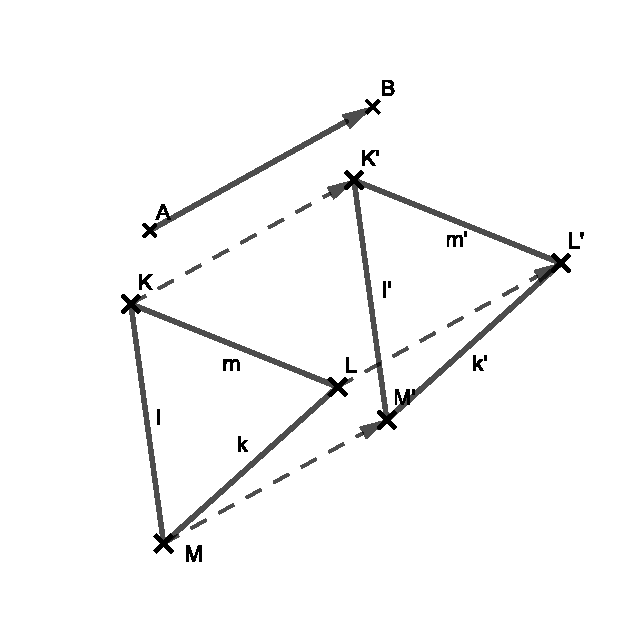
\includegraphics[width=\textwidth]{souhrn/posunuti}
\caption{$\triangle K'L'M'=\mathsf{T}_{\overrightarrow{AB}}(\triangle KLM)$}
\label{fig:posun}
\end{subfigure}
\begin{subfigure}{0.58\textwidth}
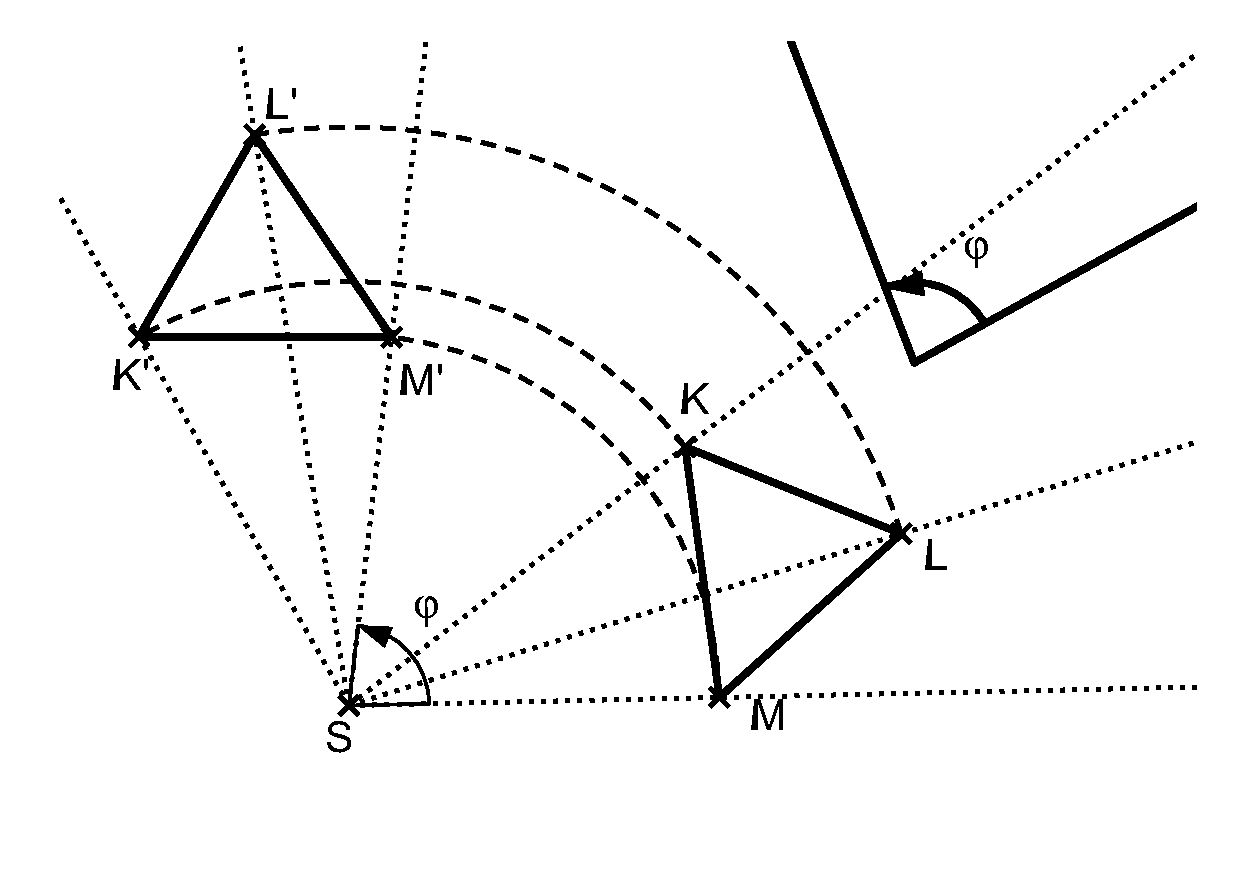
\includegraphics[width=\textwidth]{souhrn/rotace}
\caption{$\triangle K'L'M'=\mathsf{R}_{S,\varphi}(\triangle KLM)$}
\label{fig:rotace}
\end{subfigure}
\caption{Obrázky k shodným zobrazením}
\end{figure}

\chapter{Stejnolehlost}
\begin{figure}
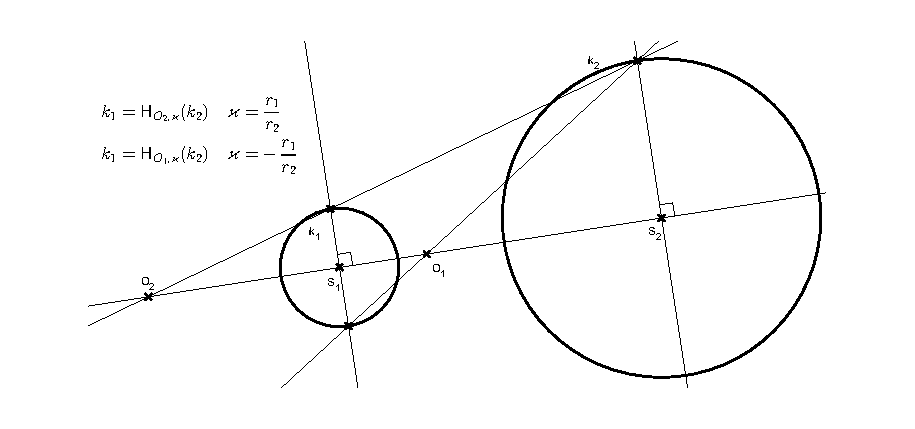
\includegraphics[width=1\textwidth]{souhrn/stejnolehlost_kruznic}
\caption{Stejnolehlost kružnic.}
\end{figure}

\chapter{Konstrukční úlohy}
\chapter{Úhly v Kružnici}

\chapter{Funkce}
\section{Úvod a pojmy}

\paragraph{Uspořádaná dvojce}
\begin{defi}%[Uspořádaná dvojce]
Uspořádaná dvojce je taková dvojce, ve které záleží na pořadí proměnných.
Platí: $ x\neq y \Rightarrow \left[ x;y \right] \neq \left[ y;x \right]$
\end{defi}

\paragraph{Kartézský součin}
\begin{defi}
Kartézský součin je množinová operace.

Kartézský součin množin $A$ a $B$, je množina \textbf{všech} uspořádaných dvojic $\left[ x;y \right]$, ve kterých $x \in A$ a zároveň $y\in B$.

$$ A\times B=\lbrace\left[x;y\right]; x\in A \wedge y\in B \rbrace $$

\end{defi}
\textbf{Pozor!} při kreslení grafů je zapotřebí dobře rozhodnout, který bod je a který není kartézským součinem. Viz \ref{fig:kartsoucin}. 
\begin{figure}[h!]
 \includegraphics[width=10cm]{souhrn/fce/bin_soucin.pdf}
 \centering
 \caption[kartézský součin graficky]{Jak ukazuje graf na obrázku, přímka zobrazující body se souřadnicí která nepatří množině je čárkovaná, každý bod na čárkované přímce nenáleží kartézskému součinu}
\label{fig:kartsoucin}
\end{figure}

\paragraph{Binární relace}
\begin{defi}
Binární relace je libovolná podmnožina kartézského součinu.
$$ U\subseteq A\times B $$
\end{defi}
\paragraph{Zobrazení}
\begin{defi}
Zobrazení je taková binární relace, která každému prvku $x\in A$ přiřazuje \textbf{nejvýš jedno} $y\in B$.
\end{defi}
\paragraph{Funkce}
\begin{defi}
Funkce je zobrazení v $\mathbb{R}$.

\textit{nebo}

Funkce je zobrazení z $\mathbb{R}$ do $\mathbb{R}$.

\end{defi}

\paragraph{Definiční obor}
\begin{defi}
$$D(f)=\left\lbrace x\in \mathbb{R};\;\exists y\in \mathbb{R};\;\left[x;y\right]\in f  \right\rbrace$$
\end{defi}\paragraph{Obor hodnot}
\begin{defi}
$$H(f)=\left\lbrace y\in \mathbb{R};\;\exists x\in \mathbb{R};\;\left[x;y\right]\in f  \right\rbrace$$
\end{defi}


\paragraph{Graf funkce $f$} je zobrazení všech bodů $X\left[x;f(x)\right],\, x\in D(f)$ do roviny.

\paragraph{} Funkce může být zadána
\begin{description}
\item[Výčtem prvků] například: $f=\lbrace [1,2],[5,7] \rbrace$
\item[Rovnicí] zápis $f:y=f(x)$
\item[Graficky] fce je vyjádřena grafem
\item[Slovním popisem] např: \emph{Funkce f každému nezápornému číslu přiřadí počet prvočísel, menších nebo rovných
tomuto číslu.}
\end{description}

\begin{defi}
Prostá funkce je taková funkce $f$. pro kterou platí:
$$ \forall x_1,\,x_2 \in D(f);\; x_1\neq x_2 \Rightarrow f(x_1)\neq f(x_2)$$

\end{defi}

\section{Vlastnosti funkcí }

\subsection{Monotónost}

Nech't $M\subseteq D(f)$.

Monotónost označuje zdali je funkce $f$ na daném intervalu rostoucí, klesající, nerostoucí, či neklesající. Monotónost lze zjistit pomocí derivace.

\begin{description}
\item[Rostoucí] na $M \Leftrightarrow \forall x_1,x_2\in M; x_1>x_2\Rightarrow f(x_1)>f(x_2)$.
\item[Klesající] na $M \Leftrightarrow \forall x_1,x_2\in M; x_1>x_2\Rightarrow f(x_1)<f(x_2)$.
\item[Neklesající] na $M \Leftrightarrow \forall x_1,x_2\in M; x_1>x_2\Rightarrow f(x_1)\geq f(x_2)$.
\item[Nerostoucí] na $M \Leftrightarrow \forall x_1,x_2\in M; x_1>x_2\Rightarrow f(x_1)\leq f(x_2)$.
\end{description}

Ryze monotónní funkce jsou funkce klesající a rostoucí.

Každá ryze monotónní funkce je zároveň prostá.

\subsection{Sudost a lichost}

Sudost a lichost jsou druhy symetrie funkcí.

\paragraph{Sudá} je funkce $\Leftrightarrow \forall x \in D(x);\; \exists -x \in D(f) \wedge f(-x)=f(x)$.

Graf takové funkce je pak osově souměrná podle osy $y$.

\paragraph{Lichá} je funkce $\Leftrightarrow \forall x \in D(x);\; \exists -x \in D(f) \wedge f(-x)=-f(x)$.

Graf funkce je pak středově souměrná podle počátku soustavy souřadnic.

\subsection{Omezenost}

Nechť $M\subseteq D(f)$.

\begin{description}
\item[Omezená zdola] je funkce $\Leftrightarrow \exists d\in \mathbb{R};\; \forall x \in M;\; f(x)>d $
\item[Omezená shora] je funkce $\Leftrightarrow \exists h \in \mathbb{R};\; \forall x \in M;\; f(x)<h$
\end{description}

Funkce je omezená na $M$ pokud je na $M$ omezená zároveň shora i zdola.

\chapter{Kombinatorika}
Kombinatorika je součást \textit{finitní} matematiky zabývající se konečnými množninami a uspořádanými $k$-ticemi (pro $k\in\mathbb{N}$)
\section{Kombinatorická pravidla}
\begin{prav}[kombinatorické pravidlo součinu]
Počet všech uspořádaných $k$-tic, jejichž první člen lze vybrat $n_1$ způsoby, druhý člen $n_2$ způsoby\dots, $k$-tý člen $n_k$ způsoby, je roven číslu $p$ pro které platí:
\end{prav}
\begin{eq}
p=n_1\cdot n_2\cdot \ldots \cdot n_k
\end{eq}


\begin{prav}[Kombinatorické pravidlo součtu]
Jsou-li $A_1,A_2\ldots A_n$ konečné množiny, které mají po řaddě $p_1,p_2\ldots p_n$ prvků, přičemž každé dvěz těchto množin jsou disjunktní, pak platí:
\begin{eq}
A_1\cup A_2\cup\ldots\cup A_n =\sum_{k=1}^{n}p_k
\end{eq}
\end{prav}
\section{Variace}
\paragraph{Variace $k$-té třídy bez opakování} $k$-člená variace z $n$ prvků ($k,n \in \mathbb{N};k\leqslant n$) je každá uspořádaná $k$-tice sestavená z těchto $n$ prvků tak, že každý se v ní vyskytuje nejvíš jednou. Počet takových variací pak je:
\begin{eq}
V_{\left(k,n\right)}=n\cdot(n-1)\cdot(n-2)\cdot\ldots\cdot(n-k+1)=\frac{n!}{(n-k)!}.
\end{eq}
Kde $V_{(k,n)}$ je \textbf{variace $k$-té třídy pro $n$ prvků bez opakování}, pokud není známo jestli s nebo bez opakování, pak se tím automaticky rozumí, že variace je bez opakování.

\paragraph{Variace $k$-té třídy s opakováním} $k$-člená variace s opakováním z $n$ prvků ($k,n \in \mathbb{N};k\leqslant n$) je každá uspořádaná $k$-tice sestavená z těchto $n$ prvků tak, že se v ní každý prvek vyskytuje nejvíše $k$-krát.
\begin{eq}
V'_{\left(k,n\right)}=n\cdot(n-1)\cdot(n-2)\cdot\ldots\cdot(n-k+1)=\frac{n!}{(n-k)!}.
\end{eq}
Kde $V_{(k,n)}$ je \textbf{variace $k$-té třídy pro $n$ prvků s opakováním}.

\section{Permutace}
\paragraph{Permutace z $n$ prvků bez opakování}
Je vlastně Variace $n$-té třídy z $n$ prvků bez opakování.

Taková permutace je uspořádaná $n$-tice sestavená z $n$ prvků tak že se v ní každý vyskytuje právě jednou. Počet takových permutací pak je:
\begin{eq}
P_{n}=V'_{\left(n,n\right)}=n\cdot(n-1)\cdot(n-2)\cdot\ldots\cdot 1=n!\,.
\end{eq}

\paragraph{Permutace s opakováním} Taková permutace je uspořádaná $n$-tice sestavená z $n$ prvků, přičemž každý je v ní obsažen nejméně jednou.

\textbf{Přesněji:} První prvek se vyskytuje $k_1$-krát, druhý $k_2$-krát,\ldots, n-tý $k_n$-krát. Pak počet takových permutací je:
\begin{eq}
P'_{k_1,k_2\ldots, k_n}(n)=\frac{n!}{k_1!\cdot k_2!\cdot\ldots\cdot k_n!}  \,.
\end{eq}

Kde $n$ je počet prvků pro něž platí $n=\sum\limits_{i=1}^{n}k_i$.

\listoffigures
\listoftables
\end{document}

\documentclass[10pt,a5paper]{article}
\usepackage[utf8]{inputenc}
\usepackage[czech]{babel}
\usepackage[T1]{fontenc}
\usepackage{amsmath}
\usepackage{amsfonts}
\usepackage{amssymb}
\usepackage{graphicx}
\usepackage{lmodern}
\usepackage[left=2cm,right=2cm,top=2cm,bottom=2cm]{geometry}
\author{Jakub Dokulil. Kateřina Kudličková}
\begin{document}
•
\end{document}
